
\chapter{Application Deployment on AWS}
\section*{Introduction}
\addcontentsline{toc}{section}{Introduction}

Cloud deployment plays a crucial role in ensuring scalability,
availability, and reliability of modern applications. In this chapter,
we present the deployment strategy of our project on Amazon Web
Services (AWS). We describe the physical and logical architecture,
the containerization process, the deployment pipeline, and the
security measures implemented to protect the system.
\newpage
\section{Project architecture}
\subsection{Physical architecture}
The physical architecture of our system consists of several interconnected layers, each serving a specific role within the overall project. Users interact with a mobile application developed in Expo, React Native, and TypeScript, providing a fluid and responsive interface for for service access.The system's core is a strong backend built with Node.js and TypeScript that manages user requests, business logic, and communication via a dedicated Python API.  A Chroma vector database, which contains all the necessary information for recommendations and optimizes user-specific suggestions, serves as the foundation for the recommendation system implemented by this Python API. Finally, all data is stored in a MongoDB database, , which guarantees the efficient and adaptable storage of user data and metadata required for the system to operate correctly.
\begin{center}
\begin{figure}[ht]
            \centering
            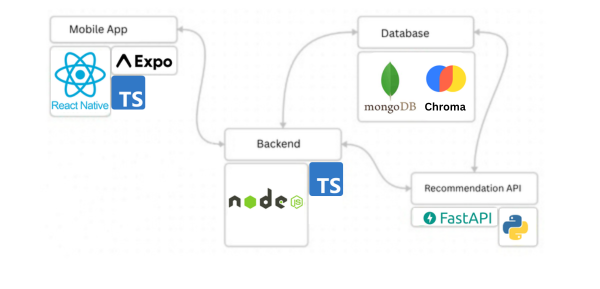
\includegraphics[scale=0.72]{images/physic_arch.png}
            \caption{Physical architecture of the system} 
            \label{fig:Physical_architecture}
        \end{figure}
\end{center}
    
\subsection{Logical architecture}

\begin{center}
\begin{figure}[ht]
            \centering
            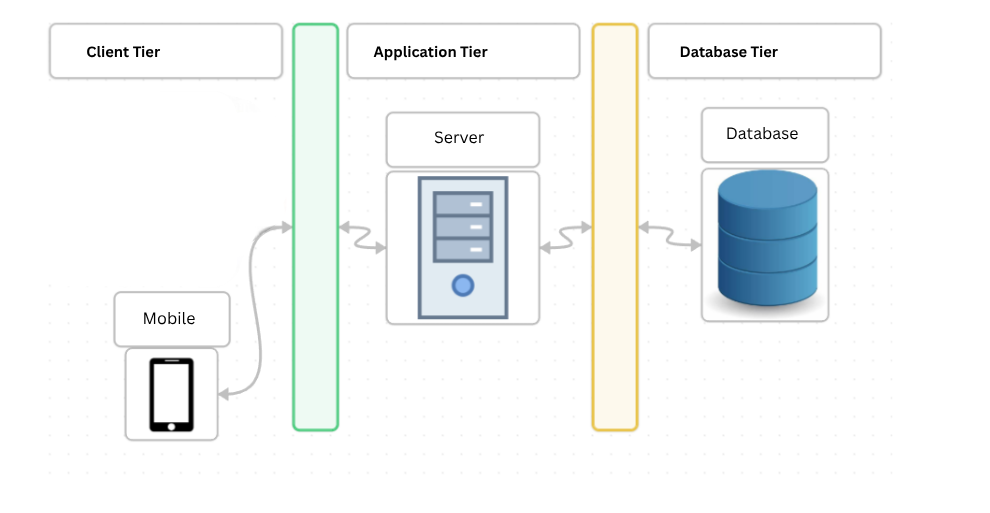
\includegraphics[scale=0.44]{images/logic_arch.png}
            \caption{Logical architecture }
            \label{fig:Logical_architecture_of_the_system}
\end{figure}
\end{center}


Our logical architecture of the system includes : a data layer, a middle layer, and a presentation layer.The data layer is responsible for information management and safe storage in an organized manner. Between the data layer and the presentation layer, the middle layer handles user requests, carries out business rules, and retrieves relevant data. The presentation layer consists of user interfaces accessible via a mobile application, enabling responsive and easy user interaction with the system.
This modular architecture enhences the scalability, maintainability, and flexibility of our application, which makes it ideal for future growth and or any adaptation.

\subsection{Containerization}
Containerization was achieved using \textbf{Docker}, which ensures
consistency across development, testing, and production
environments. Each component of the system was containerized:
\begin{itemize}
    \item \textbf{Backend (Node.js/TypeScript)} packaged as a
    container for handling API calls and business logic.
    \item \textbf{Python microservice} deployed separately to run the
    recommendation system using ChromaDB.
    \item \textbf{ChromaDB} persisted in a Docker volume to maintain
    vector embeddings.
    \item \textbf{MongoDB} containerized with persistent storage
    linked to an AWS EBS volume.
\end{itemize}

Containers communicate through a \texttt{docker-compose} network,
ensuring smooth orchestration and modular deployment.

\subsection{Deployment}
The deployment is performed on \textbf{AWS EC2}, which acts as the
compute resource for hosting the application. The architecture
includes:
\begin{itemize}
    \item An \textbf{EC2 instance} running Docker and Docker Compose.
    \item An \textbf{attached EBS volume} of 20 GB (gp3) for persistent
    storage of ChromaDB and MongoDB data.
    \item \textbf{Nginx reverse proxy} configured as an entry point to
    route traffic to the FastAPI backend, with SSL certificates managed
    by Let’s Encrypt (Certbot).
    \item Security rules applied through \textbf{AWS Security Groups}
    (see next section).
\end{itemize}

This setup allows for scalability (via Auto Scaling Groups if needed)
and ensures data persistence with EBS volumes and automated
snapshots.

\subsection{Security on Cloud}
Security is a critical aspect of cloud deployment. The following
measures were implemented:
\begin{itemize}
    \item \textbf{Security Groups:} firewall rules controlling traffic. Only
    ports 22 (SSH, restricted to admin IP), 80 (HTTP), and 443 (HTTPS)
    are open. Internal services (MongoDB, ChromaDB, FastAPI on port
    8000) remain private.
    \item \textbf{HTTPS encryption:} all traffic passes through Nginx with
    SSL/TLS enabled using Let’s Encrypt.
    \item \textbf{Data persistence:} MongoDB and ChromaDB volumes are
    stored on EBS, with daily automated snapshots for backup.
    \item \textbf{IAM roles:} AWS credentials for S3 backups and EC2
    management are restricted by least-privilege policies.
\end{itemize}

These measures ensure that the system is secure, reliable, and
compliant with industry best practices.

\section*{Conclusion}
In this chapter, we presented the deployment of our application on
AWS. We described both the physical and logical architectures, the
containerization of services using Docker, the deployment process on
EC2 with persistent EBS volumes, and the implemented security
strategies. This deployment strategy ensures that our application is
scalable, cost-effective, and secure, making it suitable for real-world
use in production.   

